
% CREACIÓN DEL DOCUMENTO
\documentclass[
	spanish, % Idioma: spanish, english, etc.
	letterpaper, oneside
]{article}

% INFORMACIÓN DEL DOCUMENTO
\def\documenttitle {Esquema de las escuelas contemporáneas de la ética}
\def\documentsubtitle {Escuelas contemporáneas de la ética}
\def\documentsubject {Actividad Semana 3}

\def\documentauthor {Martín Jonathan de la Cruz}
\def\coursename {Ética y Moral jurídica}
\def\coursecode {030}

\def\universityname {Universidad Abierta y a Distancia de México}
\def\universityfaculty {Licenciatura en Derecho}
\def\universitydepartment {Ética y Moral jurídica}
\def\universitydepartmentimage {departamentos/UnADM}
\def\universitydepartmentimagecfg {height=1.57cm}
\def\universitylocation {Roma Norte, Ciudad de México}

% INTEGRANTES, PROFESORES Y FECHAS
\def\authortable {
	\begin{tabular}{ll}
		\textbf{Alumno:}
		& \begin{tabular}[t]{l}
			 Martín Jonathan de la Cruz \\	
		\end{tabular} \\
		Matrícula: &   ES2611202040 \\
		
		\textit{Profesor:}
		& \begin{tabular}[t]{l}
			Emma Liliana \\ Padilla Cano
		\end{tabular} \\
		& \\
		\multicolumn{2}{l}{Fecha de realización: \today} \\
		% \multicolumn{2}{l}{Fecha de entrega: \today} \\
		\multicolumn{2}{l}{\universitylocation}
	\end{tabular}
}

% IMPORTACIÓN DEL TEMPLATE
\input{template}

% FORMATO SOLICITADO Y ESQUEMA TIKZ
\usepackage{helvet}
\renewcommand{\familydefault}{\sfdefault}
\usepackage{tikz}
\usetikzlibrary{arrows.meta,positioning,shadows.blur}

% CITAS EN FORMATO AUTOR-AÑO (APA)
\setcitestyle{authoryear,open={(},close={)}}

% ==============================================================================
% MARCA DE AGUA EN PORTADA
% - Se aplica solo a la portada porque usa \AddToShipoutPictureBG*.
% - Para apagarla en alguna actividad: \def\coverwatermarkenabled {false}
% - Usar opacidad baja para que no compita con titulo, datos ni logotipo.
% ==============================================================================
\def\coverwatermarkenabled {true}
\def\coverwatermarkimage {img/departamentos/UnADM.pdf}
\def\coverwatermarkopacity {0.16}
\def\coverwatermarkwidth {0.72\paperwidth}
\def\coverwatermarkxshift {0cm}
\def\coverwatermarkyshift {-0.35cm}

\newcommand{\insertcoverwatermark}{%
	\ifthenelse{\equal{\coverwatermarkenabled}{true}}{%
		\AddToShipoutPictureBG*{%
			\begin{tikzpicture}[remember picture,overlay]
				\node[
					opacity=\coverwatermarkopacity,
					inner sep=0pt,
					xshift=\coverwatermarkxshift,
					yshift=\coverwatermarkyshift
				] at (current page.center) {%
					\includegraphics[width=\coverwatermarkwidth]{\coverwatermarkimage}%
				};
			\end{tikzpicture}%
		}%
	}{}%
}

% INICIO DE PÁGINAS
\begin{document}

% PORTADA
\insertcoverwatermark
\templatePortrait

% CONFIGURACIÓN DE PÁGINA Y ENCABEZADOS
\templatePagecfg
\onehalfspacing

% RESUMEN O ABSTRACT
\begin{abstractd}
	\textbf{Objetivo:} Comprender las principales escuelas contemporáneas de la ética y su aplicación en dilemas jurídicos modernos.
 
	\textbf{Se realiza la siguiente actividad: }
Se elaboró un esquema jerárquico de seis escuelas contemporáneas de la ética --utilitarismo, ética del cuidado, neopositivismo, relativismo, neokantismo y marxismo-- desde una perspectiva filosófica. Para cada escuela se integraron definición, principios fundamentales, pregunta clave, críticas filosóficas principales y autor representativo con año clave.
\end{abstractd}

% TABLA DE CONTENIDOS - ÍNDICE
\templateIndex

% CONFIGURACIONES FINALES
\templateFinalcfg

% ======================= INICIO DEL DOCUMENTO =======================
\section{Introducción}

Una escuela ética no es una etiqueta teórica: es un criterio de decisión. En el ámbito jurídico, cada corriente define de forma distinta qué cuenta como bien, deber, verdad, justicia o responsabilidad. Por eso, comprender las escuelas contemporáneas de la ética permite identificar el sistema de razones que se activa cuando una persona, una autoridad o una institución debe decidir frente a un conflicto real.

La ética estudia racionalmente la conducta humana y la moral vivida en sociedad; no se limita a repetir costumbres, sino que analiza, ordena y critica los criterios que orientan la acción \citep{huertaEticaConClasicos2000,ronquilloarmasEticaGeneralProfesional2018}. En el Derecho, esta función es decisiva porque la norma jurídica no opera en el vacío: regula intereses, distribuye cargas, protege bienes y puede producir costos humanos. Así, las escuelas éticas sirven como modelos de lectura para responder preguntas distintas: qué consecuencia genera una decisión, qué deber debe respetarse, qué relación debe cuidarse, qué hechos pueden verificarse, qué contexto cultural condiciona el juicio y qué estructura material produce desigualdad \citep{singerCompendioEtica1995}.

El presente trabajo desarrolla un esquema de seis escuelas contemporáneas de la ética. La intención no es memorizar doctrinas, sino comparar su función: cómo ordenan el juicio moral, qué problema resuelven, qué límite presentan y qué implican para dilemas jurídicos modernos.

\section{Escuelas contemporáneas de la ética}

El utilitarismo interpreta la decisión moral desde sus consecuencias. Su criterio central es calcular qué acción produce mayor bienestar o menor sufrimiento para el conjunto. Esta escuela existe porque los conflictos sociales obligan a evaluar daños, beneficios y resultados, especialmente cuando no todas las personas pueden recibir el mismo grado de protección al mismo tiempo. Su fuerza está en mirar efectos reales; su costo filosófico aparece cuando una mayoría puede justificar el sacrificio de una minoría \citep{ronquilloarmasEticaGeneralProfesional2018,singerCompendioEtica1995}.

La ética del cuidado desplaza el centro del juicio moral: no pregunta primero por la regla abstracta ni por la utilidad total, sino por la relación concreta, la vulnerabilidad y la responsabilidad frente al otro. Su función es corregir una ética demasiado fría, incapaz de ver dependencia, afecto, acompañamiento y daño relacional. En dilemas jurídicos modernos, esta perspectiva obliga a mirar a víctimas, familias, personas vulnerables y contextos de desigualdad, no solo expedientes o categorías generales \citep{singerCompendioEtica1995}.

El neopositivismo ético sitúa el control en el lenguaje, los hechos y la verificabilidad. Su aporte consiste en exigir precisión: distinguir entre una afirmación descriptiva, una valoración moral y una emoción. Esta escuela existe como reacción contra discursos metafísicos que presentan como conocimiento lo que no puede comprobarse. Su límite es fuerte: al reducir la ética a análisis lógico o expresiones emotivas, puede dejar sin fundamento racional robusto la pregunta por el deber \citep{singerCompendioEtica1995}.

El relativismo sostiene que los juicios morales dependen de marcos culturales, históricos o subjetivos. Su valor está en impedir que una sola cultura se imponga como medida absoluta de todas las demás. Pero su riesgo es evidente: si todo depende del contexto, entonces también se debilita la posibilidad de criticar prácticas injustas desde criterios universales. En el Derecho, el relativismo sirve para contextualizar; no debe convertirse en permiso para tolerar cualquier daño \citep{singerCompendioEtica1995}.

El neokantismo recupera la fuerza del deber formal y la universalidad. Su criterio no es el resultado, sino la validez racional de la norma que guía la acción. Actuar éticamente implica respetar a la persona como fin y no como simple medio. Esta corriente aporta control normativo: una decisión jurídica no puede justificarse solo porque sea útil; debe poder defenderse como regla universal, compatible con dignidad y autonomía \citep{huertaEticaConClasicos2000,ronquilloarmasEticaGeneralProfesional2018}.

El marxismo analiza la moral desde las condiciones materiales de existencia. Su pregunta no se queda en la intención individual: examina quién posee poder, quién trabaja, quién se beneficia y quién carga el costo. Por eso su función crítica es estructural. En dilemas jurídicos, esta escuela permite observar si una norma reproduce dominación o si contribuye a transformar relaciones de explotación, exclusión o desigualdad \citep{huertaEticaConClasicos2000,ronquilloarmasEticaGeneralProfesional2018}.

\subsection{Esquema de las escuelas contemporáneas de la ética}

El esquema se organiza como una representación gráfica jerárquica de las ideas centrales de las escuelas contemporáneas de la ética según las fuentes bibliográficas: El utilitarismo, la ética del cuidado, el neopositivismo ético, el relativismo, el neokantismo y el marxismo \citep{lopezmartinezTecnicasDidacticas2023}.

\clearpage
\pagestyle{empty}
\begin{landscape}
\begin{figure}[H]
\centering
\resizebox{0.96\linewidth}{!}{%
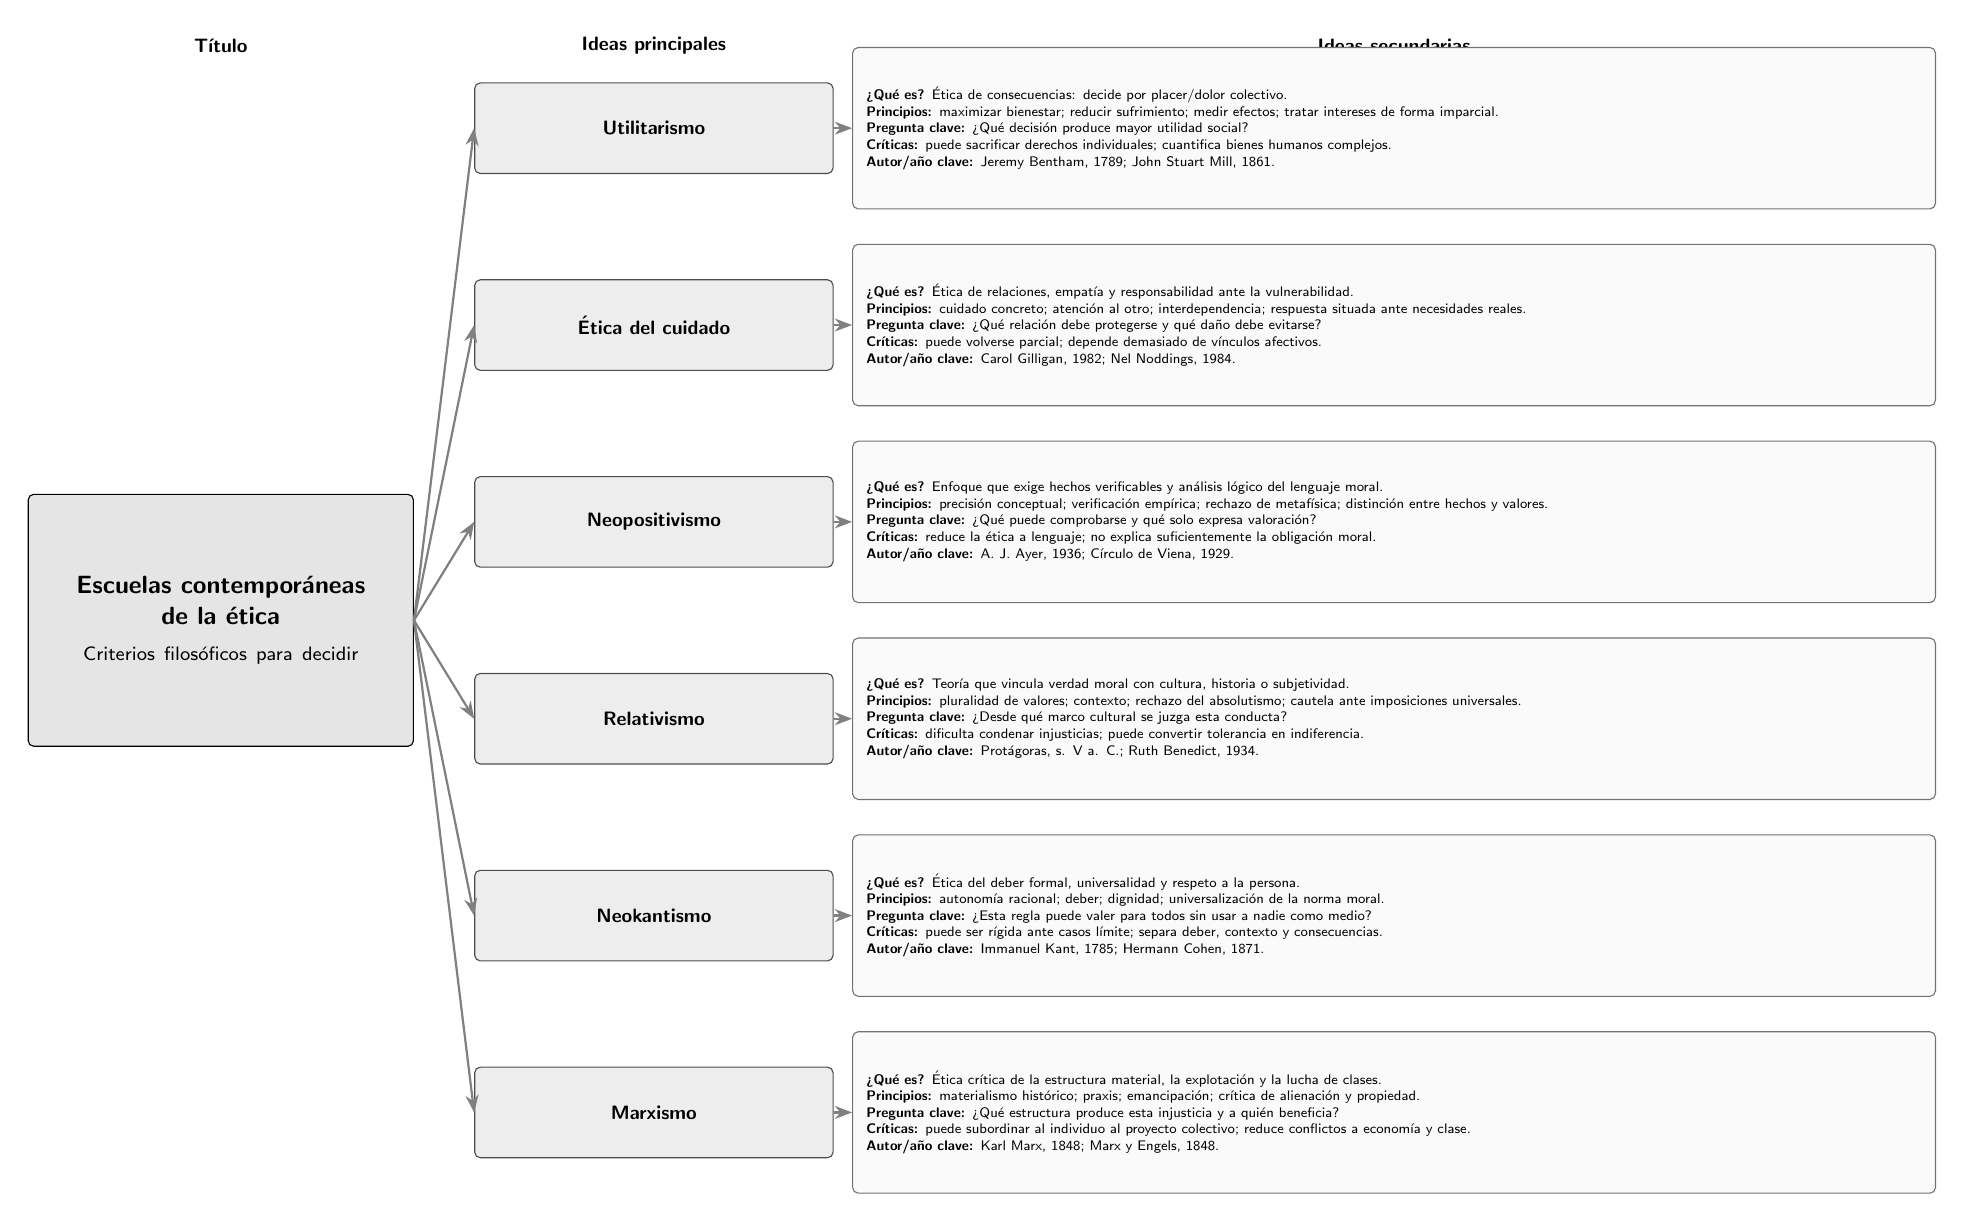
\begin{tikzpicture}[
	root/.style={
		rectangle,
		rounded corners=2pt,
		draw=black,
		fill=black!10,
		text width=4.4cm,
		minimum height=3.2cm,
		align=center,
		inner sep=7pt,
		font=\small\bfseries
	},
	main/.style={
		rectangle,
		rounded corners=2pt,
		draw=black!70,
		fill=gray!14,
		text width=4.2cm,
		minimum height=1.15cm,
		align=center,
		inner sep=5pt,
		font=\scriptsize\bfseries
	},
	detail/.style={
		rectangle,
		rounded corners=2pt,
		draw=black!55,
		fill=gray!4,
		text width=13.4cm,
		minimum height=2.05cm,
		align=left,
		inner sep=5pt,
		font=\tiny
	},
	level/.style={font=\scriptsize\bfseries, align=center},
	edge/.style={-{Stealth[length=2.2mm]}, thick, black!50}
]
\node[level] at (-6.7,1.05) {Título};
\node[level] at (-1.2,1.05) {Ideas principales};
\node[level] at (8.2,1.05) {Ideas secundarias};

\node[root] (tema) at (-6.7,-6.25) {Escuelas contemporáneas\\de la ética\\[2pt]\normalfont\scriptsize Criterios filosóficos para decidir};

\node[main] (util) at (-1.2,0) {Utilitarismo};
\node[detail] (utild) at (8.2,0) {
	\textbf{¿Qué es?} Ética de consecuencias: decide por placer/dolor colectivo.\\
	\textbf{Principios:} maximizar bienestar; reducir sufrimiento; medir efectos; tratar intereses de forma imparcial.\\
	\textbf{Pregunta clave:} ¿Qué decisión produce mayor utilidad social?\\
	\textbf{Críticas:} puede sacrificar derechos individuales; cuantifica bienes humanos complejos.\\
	\textbf{Autor/año clave:} Jeremy Bentham, 1789; John Stuart Mill, 1861.
};

\node[main] (cuidado) at (-1.2,-2.5) {Ética del cuidado};
\node[detail] (cuidadod) at (8.2,-2.5) {
	\textbf{¿Qué es?} Ética de relaciones, empatía y responsabilidad ante la vulnerabilidad.\\
	\textbf{Principios:} cuidado concreto; atención al otro; interdependencia; respuesta situada ante necesidades reales.\\
	\textbf{Pregunta clave:} ¿Qué relación debe protegerse y qué daño debe evitarse?\\
	\textbf{Críticas:} puede volverse parcial; depende demasiado de vínculos afectivos.\\
	\textbf{Autor/año clave:} Carol Gilligan, 1982; Nel Noddings, 1984.
};

\node[main] (neo) at (-1.2,-5.0) {Neopositivismo};
\node[detail] (neod) at (8.2,-5.0) {
	\textbf{¿Qué es?} Enfoque que exige hechos verificables y análisis lógico del lenguaje moral.\\
	\textbf{Principios:} precisión conceptual; verificación empírica; rechazo de metafísica; distinción entre hechos y valores.\\
	\textbf{Pregunta clave:} ¿Qué puede comprobarse y qué solo expresa valoración?\\
	\textbf{Críticas:} reduce la ética a lenguaje; no explica suficientemente la obligación moral.\\
	\textbf{Autor/año clave:} A. J. Ayer, 1936; Círculo de Viena, 1929.
};

\node[main] (rel) at (-1.2,-7.5) {Relativismo};
\node[detail] (reld) at (8.2,-7.5) {
	\textbf{¿Qué es?} Teoría que vincula verdad moral con cultura, historia o subjetividad.\\
	\textbf{Principios:} pluralidad de valores; contexto; rechazo del absolutismo; cautela ante imposiciones universales.\\
	\textbf{Pregunta clave:} ¿Desde qué marco cultural se juzga esta conducta?\\
	\textbf{Críticas:} dificulta condenar injusticias; puede convertir tolerancia en indiferencia.\\
	\textbf{Autor/año clave:} Protágoras, s. V a. C.; Ruth Benedict, 1934.
};

\node[main] (kant) at (-1.2,-10.0) {Neokantismo};
\node[detail] (kantd) at (8.2,-10.0) {
	\textbf{¿Qué es?} Ética del deber formal, universalidad y respeto a la persona.\\
	\textbf{Principios:} autonomía racional; deber; dignidad; universalización de la norma moral.\\
	\textbf{Pregunta clave:} ¿Esta regla puede valer para todos sin usar a nadie como medio?\\
	\textbf{Críticas:} puede ser rígida ante casos límite; separa deber, contexto y consecuencias.\\
	\textbf{Autor/año clave:} Immanuel Kant, 1785; Hermann Cohen, 1871.
};

\node[main] (marx) at (-1.2,-12.5) {Marxismo};
\node[detail] (marxd) at (8.2,-12.5) {
	\textbf{¿Qué es?} Ética crítica de la estructura material, la explotación y la lucha de clases.\\
	\textbf{Principios:} materialismo histórico; praxis; emancipación; crítica de alienación y propiedad.\\
	\textbf{Pregunta clave:} ¿Qué estructura produce esta injusticia y a quién beneficia?\\
	\textbf{Críticas:} puede subordinar al individuo al proyecto colectivo; reduce conflictos a economía y clase.\\
	\textbf{Autor/año clave:} Karl Marx, 1848; Marx y Engels, 1848.
};

\draw[edge] (tema.east) -- (util.west);
\draw[edge] (tema.east) -- (cuidado.west);
\draw[edge] (tema.east) -- (neo.west);
\draw[edge] (tema.east) -- (rel.west);
\draw[edge] (tema.east) -- (kant.west);
\draw[edge] (tema.east) -- (marx.west);
\draw[edge] (util.east) -- (utild.west);
\draw[edge] (cuidado.east) -- (cuidadod.west);
\draw[edge] (neo.east) -- (neod.west);
\draw[edge] (rel.east) -- (reld.west);
\draw[edge] (kant.east) -- (kantd.west);
\draw[edge] (marx.east) -- (marxd.west);
\end{tikzpicture}}
\caption{Esquema jerárquico de las escuelas contemporáneas de la ética}
\label{fig:esquema-escuelas-eticas}
\end{figure}
\end{landscape}
\pagestyle{fancy}

\subsection{Lectura jurídica del esquema}

El esquema permite ordenar las escuelas por su función. El utilitarismo decide por consecuencias; la ética del cuidado decide por responsabilidad relacional; el neopositivismo exige control del lenguaje y de los hechos; el relativismo obliga a contextualizar; el neokantismo somete la acción a deber universal; y el marxismo revela la estructura material que condiciona la moral. La diferencia no es menor: frente a un mismo dilema jurídico, cada escuela ilumina un costo distinto y también deja una zona ciega.

En una decisión jurídica moderna, utilizar solo una escuela puede producir distorsiones. El cálculo utilitarista puede justificar daños injustos; el deber formal puede ignorar desigualdades concretas; el relativismo puede debilitar la crítica; el neopositivismo puede dejar sin respuesta el sentido del deber; el cuidado puede volverse parcial; y el marxismo puede reducir la complejidad moral a conflicto estructural. Por eso, la formación jurídica exige usar estas escuelas como herramientas de análisis, no como dogmas cerrados \citep{ronquilloarmasEticaGeneralProfesional2018,singerCompendioEtica1995}.

\section{Conclusión}

Las escuelas contemporáneas de la ética muestran que decidir bien exige más que aplicar una norma: exige reconocer qué criterio moral está operando. Mi postura es que el Derecho necesita esa pluralidad para no caer en formalismo ni en cálculo frío. El jurista debe valorar consecuencias, cuidar relaciones, exigir hechos, contextualizar, respetar deberes universales y revisar estructuras de poder. Ahí la ética deja de ser teoría ornamental y se convierte en control crítico de la decisión jurídica.

\clearpage
\bibliography{EticaMoralJuridica}

% FIN DEL DOCUMENTO
\end{document}
